% stumps.tex
% Jeremy Barnes, 22/9/1999
% $Id$

\chapter{Decision Stumps}

The decision stumps algorithm is an extremely simple learning
algorithm.  As a standalone tool it is almost useless; but when
combined with the boosting algorithm it can generate very good
hypotheses.  In addition, it has a fixed VC dimension which aids in
the analysis of learning algorithms based upon it.

\section{The decision stumps learning machine}

The decision stump algorithm divides the input space
into two disjoint regions, with the boundary between them running
perpendicular to one of the axes (the decision boundary is an
axis-orthogonal hyperplane).  Each region is given a label.
Figure \ref{fig:decision stump} shows the two regions of a decision
stump classifier operating on a small, two dimensional, binary
dataset.

\begin{linefigure}
\begin{center}
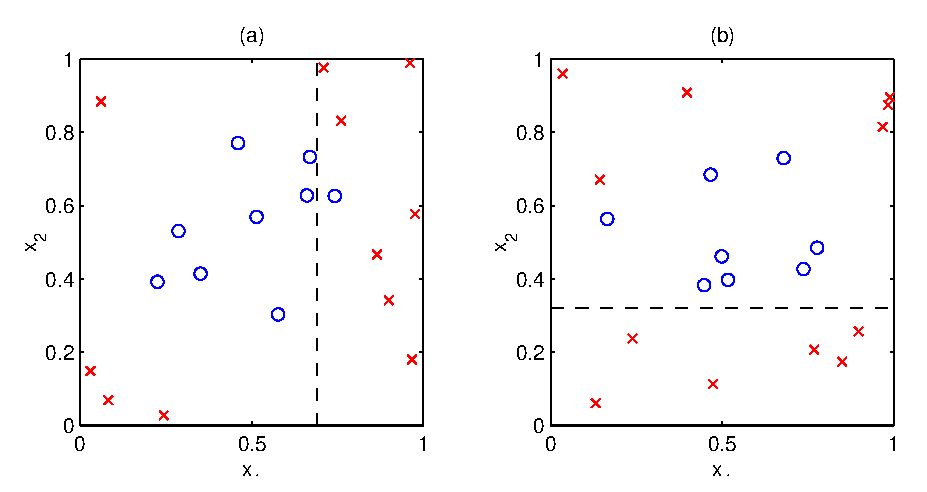
\includegraphics{figures/stumpdiagram.epsg}
\end{center}
\caption{Two decision stump classifiers.}
Both were trained on the datasets shown on the plot.  The dotted line
represents the decision boundary.  The label chosen for each region is
simply the label with the highest number of samples within that region.
\label{fig:decision stump}
\end{linefigure}

The algorithm constructs a list of possible split locations and
exhaustively searches this list for the minimum of the cost function.
Possible split locations are determined by projecting every data point
onto each axis in turn, and bisecting each pair of consecutive
projections to determine the candidate point.  See figure
\ref{fig:candidate points} for a diagram of this process.  The cost
function used is misclassifiaction risk.

\begin{linefigure}
\begin{center}
\includegraphics{figures/stumpcandidates.epsg}
\end{center}
\caption{Candidate points for decision stump split}
Data points ($\times$) are projected onto the axes.  Each consecutive
pair of projections is then bisected, to generate candidate split
points ($\bullet$).
\label{fig:candidate points}
\end{linefigure}


\section{Properties of decision stumps}

The following theorem shows that the VC dimension of decision stumps
is constant.

\begin{theorem}[VC dimension of decision stumps]
\label{theorem:vcdim stumps}
The set $\mathcal{S}$ of decision stump classifiers on an domain
$\calI$ has a VC dimension of
%
\begin{equation}
\VCdim(\calS) = 2
\end{equation}
%
\proof Consider figure \ref{fig:stump vc dim proof}.  It is obvious
from the figure that any two points that are not coincident can be
shattered by the decision stump.  It is also obvious that there is no
set of three points that can be shattered by the decision stump.  It
is also obvious that this will hold for any number of dimensions.
Thus, $\VCdim(\calS) = 2$.
\end{theorem}

\begin{linefigure}
\begin{center}
\includegraphics{figures/stumpvcdim.epsg}
\end{center}
\caption{Candidate points for decision stump split}
Part (a) shows how any two points can be shattered by a decision
stump.  Part (b) shows how no three points can be shattered by a
decision stump.
\label{fig:stumps vc dim proof}
\end{linefigure}

This result is useful as it can be applied to bounds in \ref{??} to
calculate the performance of algorithms.




